\let\negmedspace\undefined
\let\negthickspace\undefined
\documentclass[journal]{IEEEtran}
\usepackage[a5paper, margin=10mm, onecolumn]{geometry}
%\usepackage{lmodern} % Ensure lmodern is loaded for pdflatex
\usepackage{tfrupee} % Include tfrupee package

\setlength{\headheight}{1cm} % Set the height of the header box
\setlength{\headsep}{0mm}  % Set the distance between the header box and the top of the text

\usepackage{gvv-book}
\usepackage{gvv}
\usepackage{cite}
\usepackage{amsmath,amssymb,amsfonts,amsthm}
\usepackage{algorithmic}
\usepackage{graphicx}
\usepackage{textcomp}
\usepackage{xcolor}
\usepackage{txfonts}
\usepackage{listings}
\usepackage{enumitem}
\usepackage{mathtools}
\usepackage{gensymb}
\usepackage{comment}
\usepackage[breaklinks=true]{hyperref}
\usepackage{tkz-euclide} 
\usepackage{listings}
% \usepackage{gvv}                                        
\def\inputGnumericTable{}                                 
\usepackage[latin1]{inputenc}                                
\usepackage{color}                                            
\usepackage{array}                                            
\usepackage{longtable}                                       
\usepackage{calc}                                             
\usepackage{multirow}                                         
\usepackage{hhline}                                           
\usepackage{ifthen}                                           
\usepackage{lscape}
\begin{document}

\bibliographystyle{IEEEtran}
\vspace{3cm}

\title{1.9.3}
\author{EE24BTECH11021 - Eshan Ray}

% \maketitle
% \newpage
% \bigskip
{\let\newpage\relax\maketitle}

\renewcommand{\thefigure}{\theenumi}
\renewcommand{\thetable}{\theenumi}
\setlength{\intextsep}{10pt} % Space between text and floats




\textbf{Question: }\\
AOBC is a rectangle whose three vertices are \brak{0, -3}, \brak{0, 0} and \brak{4, 0}. The length of
its diagonal is\dots \\
\solution {
\begin{table}[h!]    
  \centering
  \begin{tabular}[12pt]{ |c| c|}
    \hline
        \textbf{Variable}  & \textbf{Description} \\
    \hline
        $\vec{B}$$\brak{-4,0}$ &  coordinates of first point  \\
    \hline 
        $\vec{C}$$\brak{10,0}$ & coordinates of second point \\
    \hline
        $\vec{A}$& Equidistant point of $\vec{B}$ and $\vec{C}$ on $X$ axis \\  
    \hline
         
\end{tabular}

  \caption{Input parameters}
  \label{tab1.1.9.2}
\end{table}

   In a rectangle any $3$ adjacent points form a right triangle, where the hypotenuse is the diagonal.\\
    So, in $\triangle AOB$,
    \begin{align}
         l &= \norm{\vec A -\vec B}\\
        \implies l&= \sqrt{\brak{\vec A-\vec B}^\top\brak{\vec A-\vec B}}\\
        \implies l&= \sqrt{\myvec{-4 & -3}\myvec{-4\\-3}}\\
        \implies l&= \sqrt{25}\\
        \implies l&= 5\\
        Similarly,a&=\norm{\vec B-\vec O}\\
        \implies a&=\sqrt{\brak{4^2}}\\
        \implies a&= 4\\
        and,b&= \norm{\vec A-\vec O}\\
        \implies b&=\sqrt{\brak{3^2}}\\
        \implies b&=3
    \end{align}
     $l=5$ is the greatest length of $\triangle AOB$.\\
    $\therefore$ The length of diagonal of rectangle $AOBC$ = $5$.
    \begin{figure}[!ht]
    \centering
	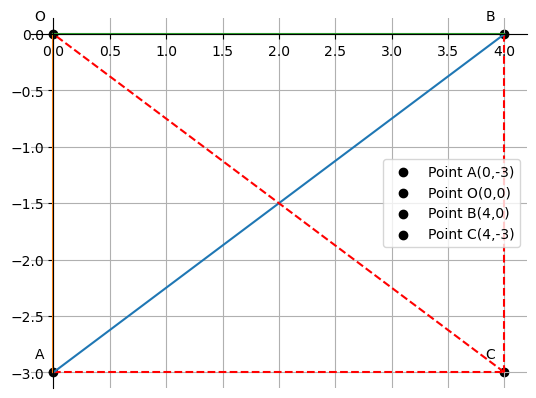
\includegraphics[width=1\textwidth]{plots/plot.png}
    \caption{}
    \label{fig:plot}
\end{figure}  
}
\end{document}


